%%%%%%%%%%%%%%%%%%%%%%%%%%%%%%%%%%%%%%%%%
% In-class Quiz #2 Template
% LaTeX Template
% By: Ryan Grove
%%%%%%%%%%%%%%%%%%%%%%%%%%%%%%%%%%%%%%%%%

%----------------------------------------------------------------------------------------
%	PACKAGES AND OTHER DOCUMENT CONFIGURATIONS
%----------------------------------------------------------------------------------------

\documentclass[paper=a4, fontsize=11pt]{scrartcl} % A4 paper and 11pt font size

\usepackage[T1]{fontenc} % Use 8-bit encoding that has 256 glyphs
\usepackage{fourier} % Use the Adobe Utopia font for the document - comment this line to return to the LaTeX default
\usepackage[english]{babel} % English language/hyphenation
\usepackage{amsmath,amsfonts,amsthm} % Math packages

\usepackage{lipsum} % Used for inserting dummy 'Lorem ipsum' text into the template

\usepackage{sectsty} % Allows customizing section commands
\allsectionsfont{\centering \normalfont\scshape} % Make all sections centered, the default font and small caps

\usepackage{fancyhdr} % Custom headers and footers
\pagestyle{fancyplain} % Makes all pages in the document conform to the custom headers and footers
\fancyhead{} % No page header - if you want one, create it in the same way as the footers below
\fancyfoot[L]{} % Empty left footer
\fancyfoot[C]{} % Empty center footer
%\fancyfoot[R]{\thepage} % Page numbering for right footer
\renewcommand{\headrulewidth}{0pt} % Remove header underlines
\renewcommand{\footrulewidth}{0pt} % Remove footer underlines
\setlength{\headheight}{13.6pt} % Customize the height of the header

\numberwithin{equation}{section} % Number equations within sections (i.e. 1.1, 1.2, 2.1, 2.2 instead of 1, 2, 3, 4)
\numberwithin{figure}{section} % Number figures within sections (i.e. 1.1, 1.2, 2.1, 2.2 instead of 1, 2, 3, 4)
\numberwithin{table}{section} % Number tables within sections (i.e. 1.1, 1.2, 2.1, 2.2 instead of 1, 2, 3, 4)

\setlength\parindent{0pt} % Removes all indentation from paragraphs - comment this line for an assignment with lots of text

\usepackage{lastpage}
\usepackage{fancyhdr}
\cfoot{\thepage\ of \pageref{LastPage}}

\usepackage{graphicx}

%----------------------------------------------------------------------------------------
%	TITLE SECTION
%----------------------------------------------------------------------------------------

\newcommand{\horrule}[1]{\rule{\linewidth}{#1}} % Create horizontal rule command with 1 argument of height

\title{	
\normalfont \normalsize 
\textsc{Ryan Grove, Clemson University, MATH1080 - 9} \\ [25pt] % Your name, university, class
\horrule{0.5pt} \\[0.4cm] % Thin top horizontal rule
\huge In-class Quiz \#2 \\ % The assignment title
\horrule{2pt} \\[0.5cm] % Thick bottom horizontal rule
}

\author{Date:} % The due date

\date{\normalsize January 15, 2016} % A custom date

\begin{document}

\maketitle % Print the title

\begin{flushleft}
\begin{tabular}{l l}
Name: \rule{3.2in}{.01cm}  & {}%Table number: \rule{1in}{.01cm}\\
\end{tabular}
\end{flushleft}

%----------------------------------------------------------------------------------------
%	Directions
%----------------------------------------------------------------------------------------

\section*{\textbf{Directions:}}

No calculator or notes may be used.  Read each question very carefully.  In order to receive full credit, you must:
\begin{enumerate}
\item Show legible and logical (relevant) justification which supports your final answer.
\item Use complete and correct mathematical notation.
\item Include proper units, if necessary.
\item Give exact numerical values whenever possible.
\item Follow the directions given for the problem.
\end{enumerate}
\vspace{.1in}

\newpage

\begin{enumerate}
\setlength{\itemsep}{0.45in}
\item (2 points) Sketch the region enclosed by the given curves.  Decide whether to integrate with respect to $x$ or $y$.  \textbf{HINT:} Draw a typical approximating triangle and label its height and width.  Then find the area of the region.\\

The curves are $\displaystyle y=(x-2)^2 \text{ and } y=x$\\

\noindent\textbf{Solution:}\\
The points of intersection are found as follows:
\begin{align*}
(x-2)^2 &= x \\
\implies x^2 -4x + 4 &= x\\
\implies x^2 - 5x + 4 &= 0\\
\implies (x-1)(x-4) &= 0\\
\implies x &= 1,4
\end{align*}

Now, we can find the area as follows:
\begin{align*}
A(x) &= \int_1^4 \left( (x) - (x-2)^2 \right) \text{  } dx \\
&= \int_1^4 \left( (x) - (x^2-4x+4) \right) \text{  } dx \\
&= \int_1^4 \left( (x) - (x^2 - 5x + 4) \right) \text{  } dx \\
&= \left[ -\frac{1}{3}x^3 + \frac{5}{2}x^2 - 4x\right]_1^4\\
&= \boxed{\frac{9}{2}}
\end{align*}

\item (2 points) Find the volume of the solid obtained by rotating the region bounded by the given curves about the specified line.  \textbf{HINT:} Sketch the region, the solid, and a typical disk or washer.\\

The region is $\displaystyle y=x^3, y=x, x \ge 0$ about the $x$-axis

\noindent\textbf{Solution:}\\
We find the area as follows:
\begin{align*}
A(x) &= \pi R^2 - \pi r^2\\
&= \pi x^2 - \pi x^6
\end{align*}

Now, we can find the volume as follows:
\begin{align*}
V(x) &= \int_0^1 A(x) \text{  } dx \\
&= \int_0^1 \left( \pi x^2 - \pi x^6 \right) \text{  } dx \\
&=  \pi  \int_0^1  \left(x^2 - x^6 \right) \text{  } dx \\
&=   \pi \left[ \frac{1}{3}x^3 - \frac{1}{7}x^7 \right]_0^1\\
&= \boxed{ \frac{4 \pi}{21} }
\end{align*}

\item (2 points) Use the method of cylindrical shells to find the volume generated by rotating the region bounded by the given curves about the y-axis.\\

\noindent\textbf{Solution:}\\
The point of intersection is $(2,4)$.

Now, we can find the volume as follows:
\begin{align*}
V(x) &= \int_0^2 2 \pi (x) \left( (6x-2x^2)-(x^2) \right)  \text{  } dx \\
&= 2 \pi \int_0^2  \left( 6x^2-3x^3 \right)  \text{  } dx \\
&= 2 \pi \left[ 2x^3 - \frac{3}{4}x^4 \right]_2^6\\
&= \boxed{8 \pi}
\end{align*}
\newpage
\item (4 points) Consider the region bounded by $x=2y$ and $x=y^2$.\\
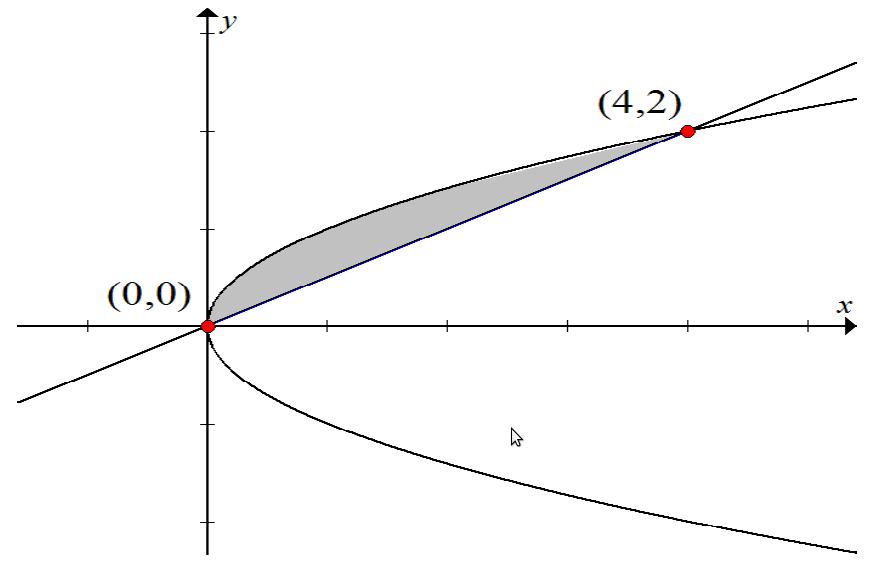
\includegraphics[width=11cm]{IC2_4}\\
Answer the following questions on the next page. 

Set up, but \textbf{DO NOT} evaluate or simplify, the integral expression for the volume obtained by rotating this region about the specified axis, using the given method.\\
\begin{enumerate}
\item Shell method about $x=-1$.\\
\noindent\textbf{Solution:}\\
$ V = \boxed{ \int_0^4 2 \pi (1+x) \left( \sqrt{x} - \frac{1}{2}x \right) \text{  } dx}$
\item Disk/washer method about $x=-1$.\\
\noindent\textbf{Solution:}\\
$V = \boxed{\int_0^2 \pi \left[ (1+2y)^2 - (1+y^2)^2 \right] \text{  } dy}$
\item Shell method about $y=3$.\\
\noindent\textbf{Solution:}\\
$V =\boxed{\int_0^2 2 \pi (3-y)(2y-y^2) \text{  } dx}$
\item Disk/washer method about $y=-2$.\\
\noindent\textbf{Solution:}\\
$V = \boxed{\int_0^4  \pi  \left[ (2+\sqrt{x})^2 - \left (2+\frac{1}{2}x \right)^2 \right] \text{  } dy}$
\end{enumerate}




\end{enumerate}

%----------------------------------------------------------------------------------------

\end{document}